\section{Sensitivity}\label{section:sensitivity}

Sensitivity \cite{yeh2019fidelity} (\textit{max-sensitivity} to be precise) is defined as a measure of change in the attribution with a small perturbation to the input.


\begin{definition}[Sensitivity]\label{def:sensitivity}
    For a given model $F$, attribution method $\Phi$, input $x$, insignificant perturbation $\delta$, and input neighborhood radious $r$, \textit{max-sensitifity} for a attribution is defined as:
    
    \begin{equation}
        \operatorname{SENS}_{\operatorname{MAX}}(\Phi, \mathbf{F}, \mathbf{x}, r):=\max _{\|\mathbf{\delta}\| \leqslant r} \| \Phi(\mathbf{F}, \mathbf{x} + \mathbf{\delta})-\Phi(\mathbf{F}, \mathbf{x}) \|
        \label{eq:sensitivity}
    \end{equation}
\end{definition}

\begin{wrapfigure}{L}{0.35\textwidth}
  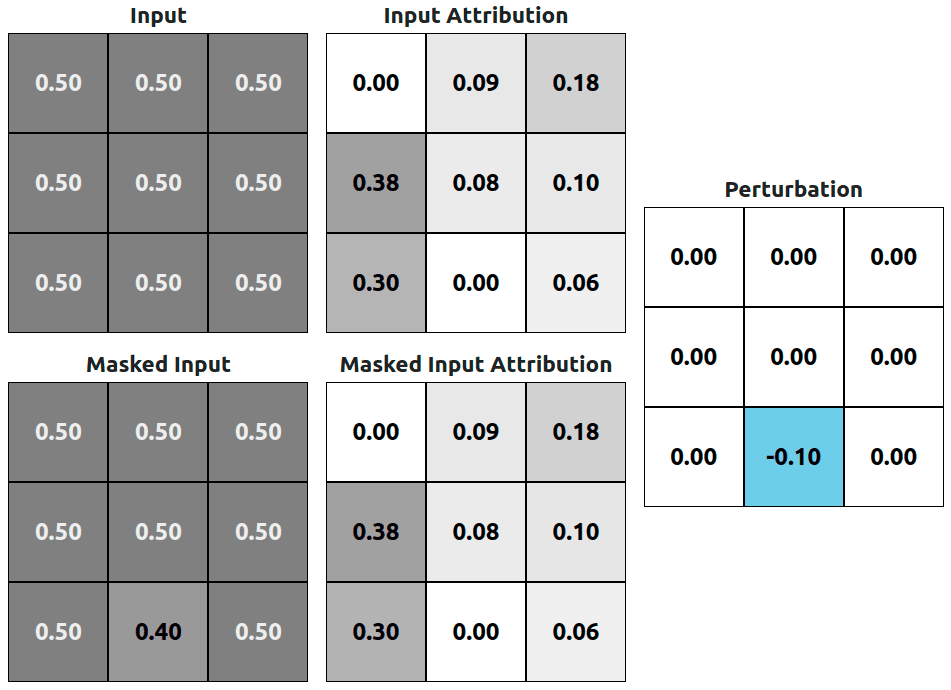
\includegraphics[width=0.35\textwidth]{methods/images/same-sens.png}
  \caption{\textbf{Sensitivity = 0}. Perturbation of the input did not change the attribution between the input and masked input (one with added perturbation).}\label{fig:sensitivyt-same}
  \smallskip\par
  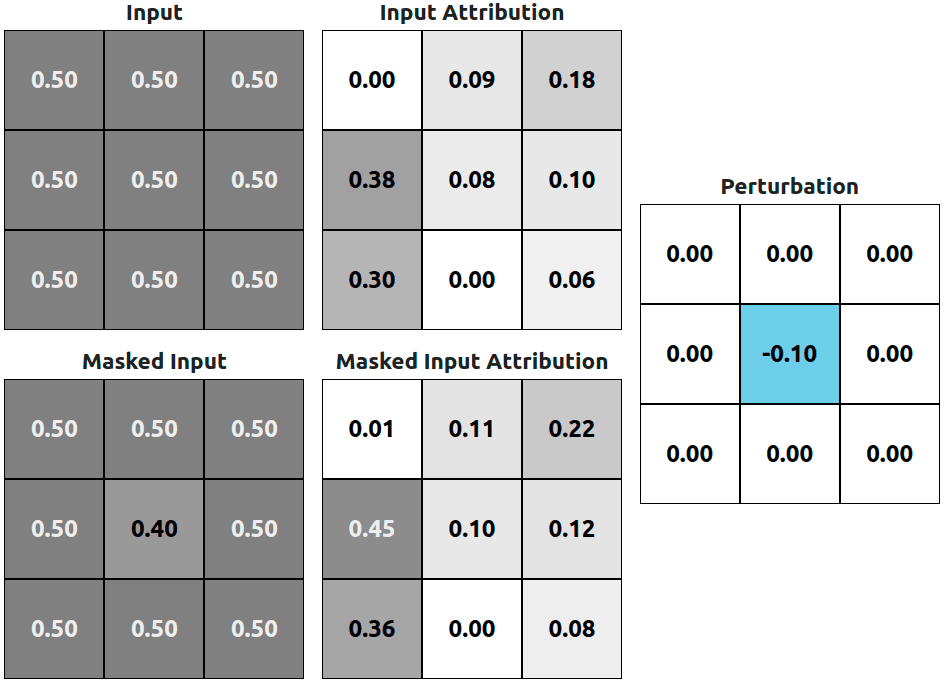
\includegraphics[width=0.35\textwidth]{methods/images/change-sens.png}
  \caption{\textbf{Sensitivity = 0.11}. Perturbation of the feature with higher than zero initial attribution causes Sensitivity value to rise.}\label{fig:sensitivyt-change}
\end{wrapfigure}


The radius $r$ serves as a radius of a $l_p norm$ used to generate insignificant perturbation. It restricts the range of the perturbation and usually is set to around $0.02$. Sensitivity returns a positive scalar which is the length of the sensitivity vector. This vector (as shown in eq. \ref{eq:sensitivity}) is the difference between two attribution vectors, so the absolute length of this vector is proportional to the difference in every dimension of the attribution vectors.



\vspace{2\baselineskip}

To explain the intuition behind the sensitivity, we can use a toy example of the model that takes $3x3$ input and predicts the class $[0,1]$. This model predicts class $0$ with a $0.95$ score when receiving the input filled with $0.50$. Attribution for this prediction is shown in Figure \ref{fig:sensitivyt-same} (Input Attribution). If a perturbation is added to the input, then new attribution is calculated for the same class ($0$) but for the \textit{Masked Input}. If the perturbation doesn't affect the attribution (as in Fig. \ref{fig:sensitivyt-same}), then returned Sensitivity measure is equal to zero.

\vspace{\baselineskip}

It is common for attribution to remain constant when perturbing features of the input with initial attribution close to zero. Attribution defines how much specific feature is involved in the model decision. Changing the value, which is irrelevant for the model, usually results in close to no change in the attribution.

\vspace{\baselineskip}

An example that causes the $\operatorname{SENS}$ value to change can be seen in Figure \ref{fig:sensitivyt-change}. This time perturbation changes the feature with non-zero attribution of the original input (\textit{Input Attribution}). That perturbation causes the new attribution (\textit{Masked Input Attribution}) to differ slightly from the original one. The length of the vector (total difference between two attributions) is equal to $0.11$ which is a square root of squared differences between corresponding attribution positions.

\vspace{\baselineskip}

\textbf{Remark.} Perturbation shown in the example is created for the purpose of the example. In practice, values in the perturbation will be significantly smaller and will affect the whole input, not only one feature.